\documentclass[11pt,a4paper]{article}

\usepackage[utf8]{inputenc}
\usepackage[T1]{fontenc}
\usepackage[spanish,es-nodecimaldot]{babel}
\usepackage{amsmath}
\usepackage{booktabs}
\usepackage{tabularx}
\usepackage{array}
\usepackage{graphicx}
\usepackage{geometry}
\usepackage{xcolor}
\usepackage{float}
\usepackage{caption}
\usepackage{hyperref}
\geometry{margin=2.2cm}

\hypersetup{
    colorlinks=true,
    linkcolor=blue!50!black,
    urlcolor=blue!50!black,
    pdftitle={Reporte de auditoria de corrida larga residual},
    pdfauthor={Cesar Zapata}
}

\newcolumntype{Y}{>{\raggedright\arraybackslash}X}

\title{Reporte de auditor\'ia de corrida larga residual\\\large Proyecto TD3 para pr\'otesis mioel\'ectrica}
\author{C\'esar Zapata\\Research Laboratory in Artificial Intelligence and Computer Vision ``Alan Turing''}
\date{2 de abril de 2026}

\begin{document}
\maketitle

\section*{Prop\'osito}
Este documento resume la auditor\'ia completa, el test final y la interpretaci\'on t\'ecnica de la corrida larga residual \texttt{26-04-01 19 14 56}. La motivaci\'on de esta corrida no fue producir nueva evidencia estad\'istica de robustez, sino observar qu\'e ocurr\'ia si la l\'inea residual se segu\'ia entrenando mucho m\'as all\'a de las corridas previas de 2000 episodios.

La pregunta concreta fue simple: \emph{si se extiende el entrenamiento residual hasta 50000 episodios, aparece un checkpoint mejor que los candidatos ya conocidos o el agente deriva hacia un compromiso peor?}

\section*{Punto de partida del proyecto}
Antes de esta corrida, el estado del proyecto estaba resumido as\'i:
\begin{itemize}
    \item \textbf{Benchmark oficial estable:} \texttt{Agent7250}.
    \item \textbf{Mejor residual single-run hist\'orico:} \texttt{Agent1850}, con mejora fuerte de esfuerzo y saturaci\'on, pero sin evidencia robusta entre seeds.
    \item \textbf{Mejor residual reproducible:} la \texttt{seed 22} de la campa\~na multi-seed, que fue la \'unica aceptada bajo \texttt{ConditionA}.
\end{itemize}

Por lo tanto, la corrida larga se interpret\'o desde el inicio como una \textbf{exploraci\'on futura del residual}, no como reemplazo autom\'atico del benchmark.

\section*{Configuraci\'on heredada de la corrida larga}
La corrida larga mantuvo exactamente la receta residual final y solo ampli\'o la duraci\'on temporal del entrenamiento.

\begin{table}[H]
\centering
\caption{Configuraci\'on principal de la corrida larga residual}
\begin{tabularx}{\linewidth}{lY}
\toprule
Elemento & Valor \\
\midrule
Carpeta experimental & \texttt{Agentes/agente\_corrida\_larga26-04-01 19 14 56} \\
Agente & \texttt{td3\_residual\_lift} \\
Checkpoint base congelado & \texttt{Agent7250} \\
Escala residual & $\alpha_{\mathrm{res}} = 0.20$ \\
Exploraci\'on & $0.02 / 0.002 / 10^{-4}$ \\
Episodios de entrenamiento & 50000 \\
Guardado de checkpoints & cada 500 episodios \\
Guardado de episodios & cada 500 episodios \\
Plots de entrenamiento & \texttt{none} \\
Semilla aleatoria controlada & no (\texttt{randomSeed = NaN}) \\
\bottomrule
\end{tabularx}
\end{table}

\section*{Qu\'e se quiso observar}
La corrida se lanz\'o para ver si una extensi\'on temporal muy larga pod\'ia producir alguno de estos tres escenarios:
\begin{enumerate}
    \item una mejora sostenida respecto a las corridas residuales cortas;
    \item una meseta temprana, donde seguir entrenando ya no aportara valor;
    \item una deriva tard\'ia, donde el agente aprendiera soluciones cada vez menos estables o m\'as agresivas.
\end{enumerate}

Como esta pregunta mira toda la trayectoria y no solo la cola del entrenamiento, la auditor\'ia posterior se defini\'o sobre \textbf{todos los checkpoints guardados}.

\section*{Lectura del entrenamiento}
La Fig.~\ref{fig:training} resume el \texttt{training\_info.mat} de la corrida.

\begin{figure}[H]
\centering
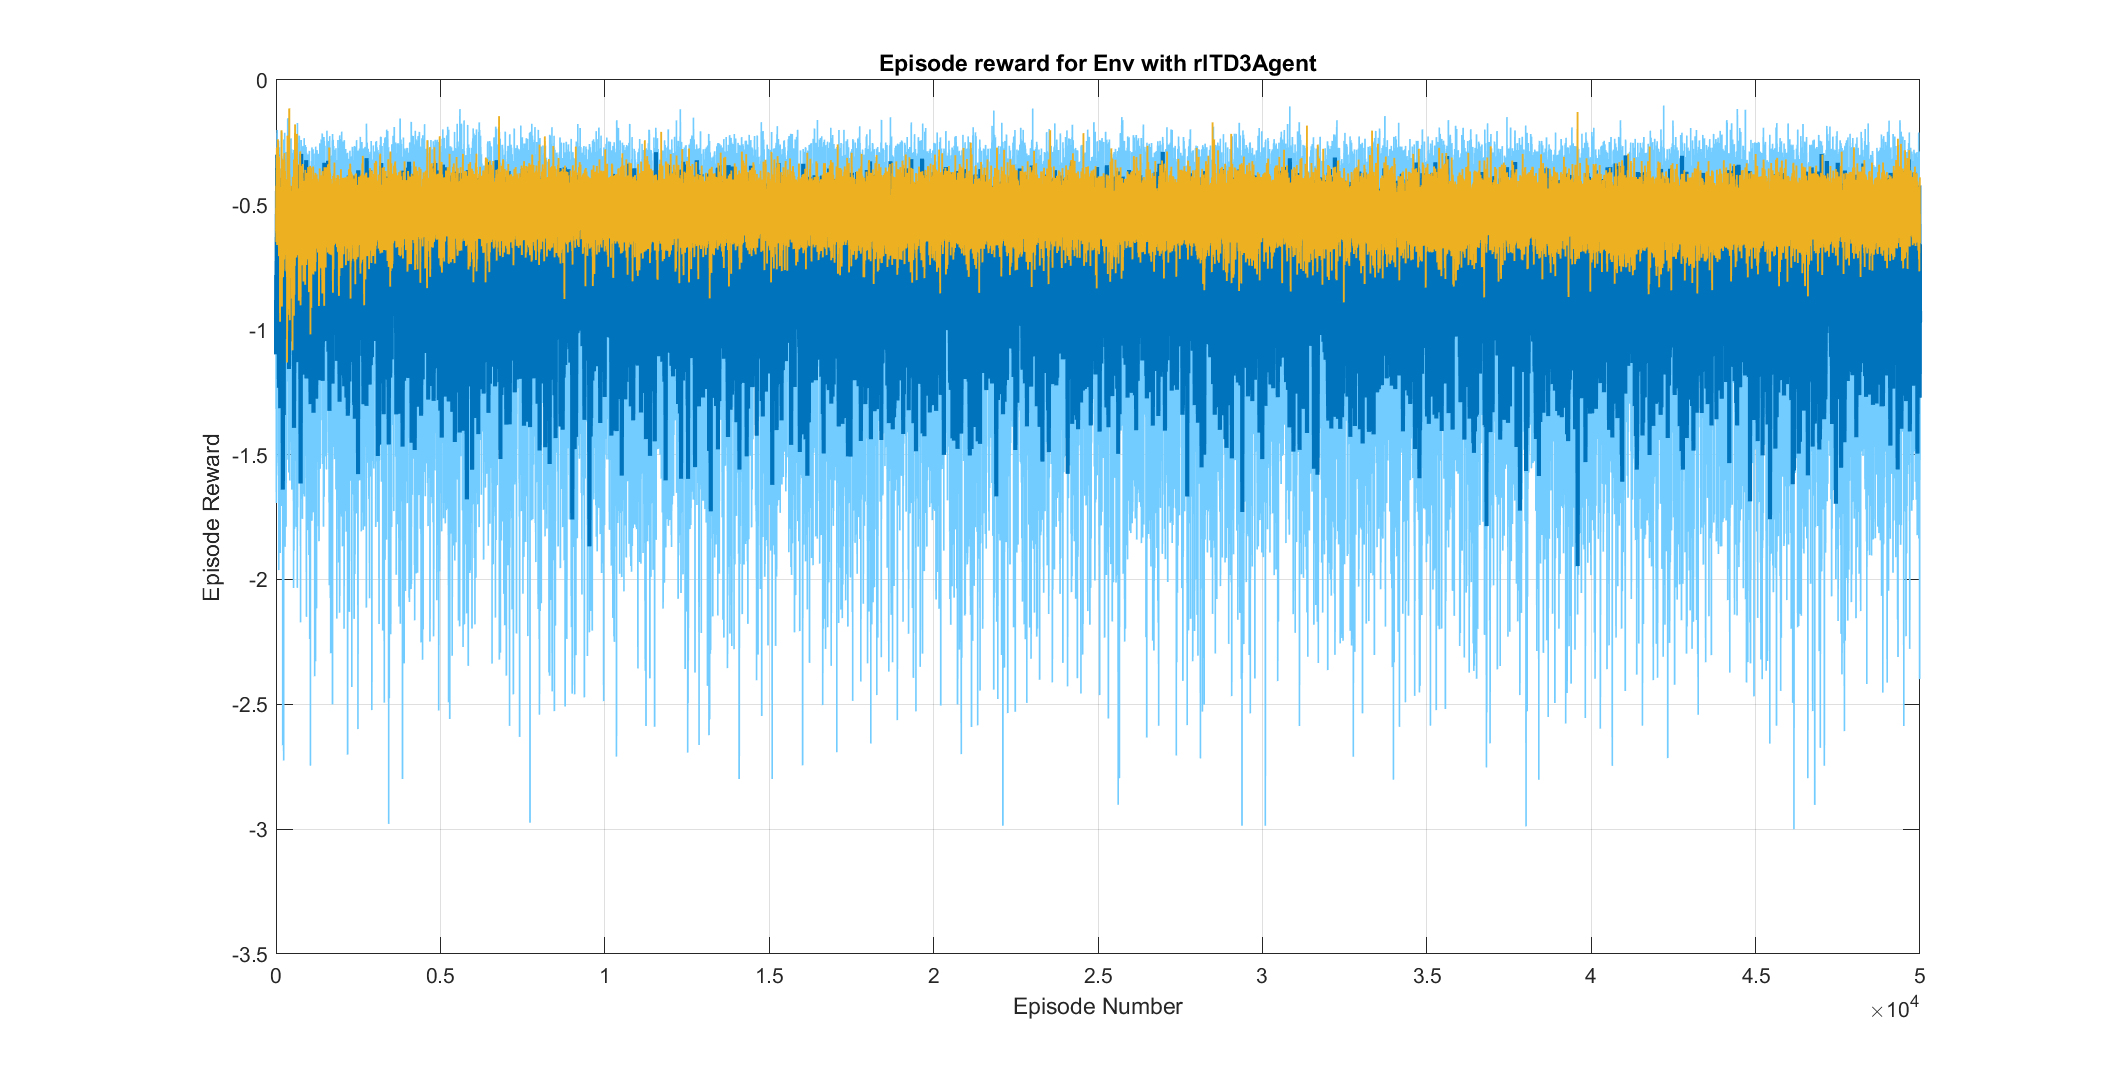
\includegraphics[width=\linewidth]{figures/longrun_residual_training_progress_20260402.png}
\caption{Resumen del entrenamiento largo residual. Se muestran \texttt{EpisodeReward}, \texttt{AverageReward} y \texttt{EpisodeQ0} a lo largo de 50000 episodios.}
\label{fig:training}
\end{figure}

Los datos principales del entrenamiento fueron:
\begin{itemize}
    \item episodios totales: 50000;
    \item \texttt{AverageReward} final: \(-0.970405\);
    \item mejor \texttt{AverageReward}: \(-0.287762\);
    \item episodio del mejor \texttt{AverageReward}: 26969;
    \item \texttt{TotalAgentSteps} final: 711878.
\end{itemize}

La lectura t\'ecnica es clara: el entrenamiento no mostr\'o mejora sostenida hasta el final. El mejor comportamiento medio apareci\'o aproximadamente a la mitad de la corrida y despu\'es se observ\'o deterioro. En otras palabras, la extensi\'on temporal larga no consolid\'o el agente; m\'as bien introdujo evidencia de \textbf{deriva tard\'ia}.

\section*{Auditor\'ia completa de checkpoints}
Se audit\'aron los 100 checkpoints guardados, desde \texttt{Agent500.mat} hasta \texttt{Agent50000.mat}, con el mismo protocolo de dos fases usado en etapas anteriores:
\begin{itemize}
    \item fase r\'apida: 20 simulaciones;
    \item fase completa: 50 simulaciones;
    \item ranking por compromiso entre error de seguimiento, esfuerzo de acci\'on, saturaci\'on y suavidad de acci\'on;
    \item selecci\'on final del mejor checkpoint por la tabla \texttt{phaseB}.
\end{itemize}

\begin{figure}[H]
\centering
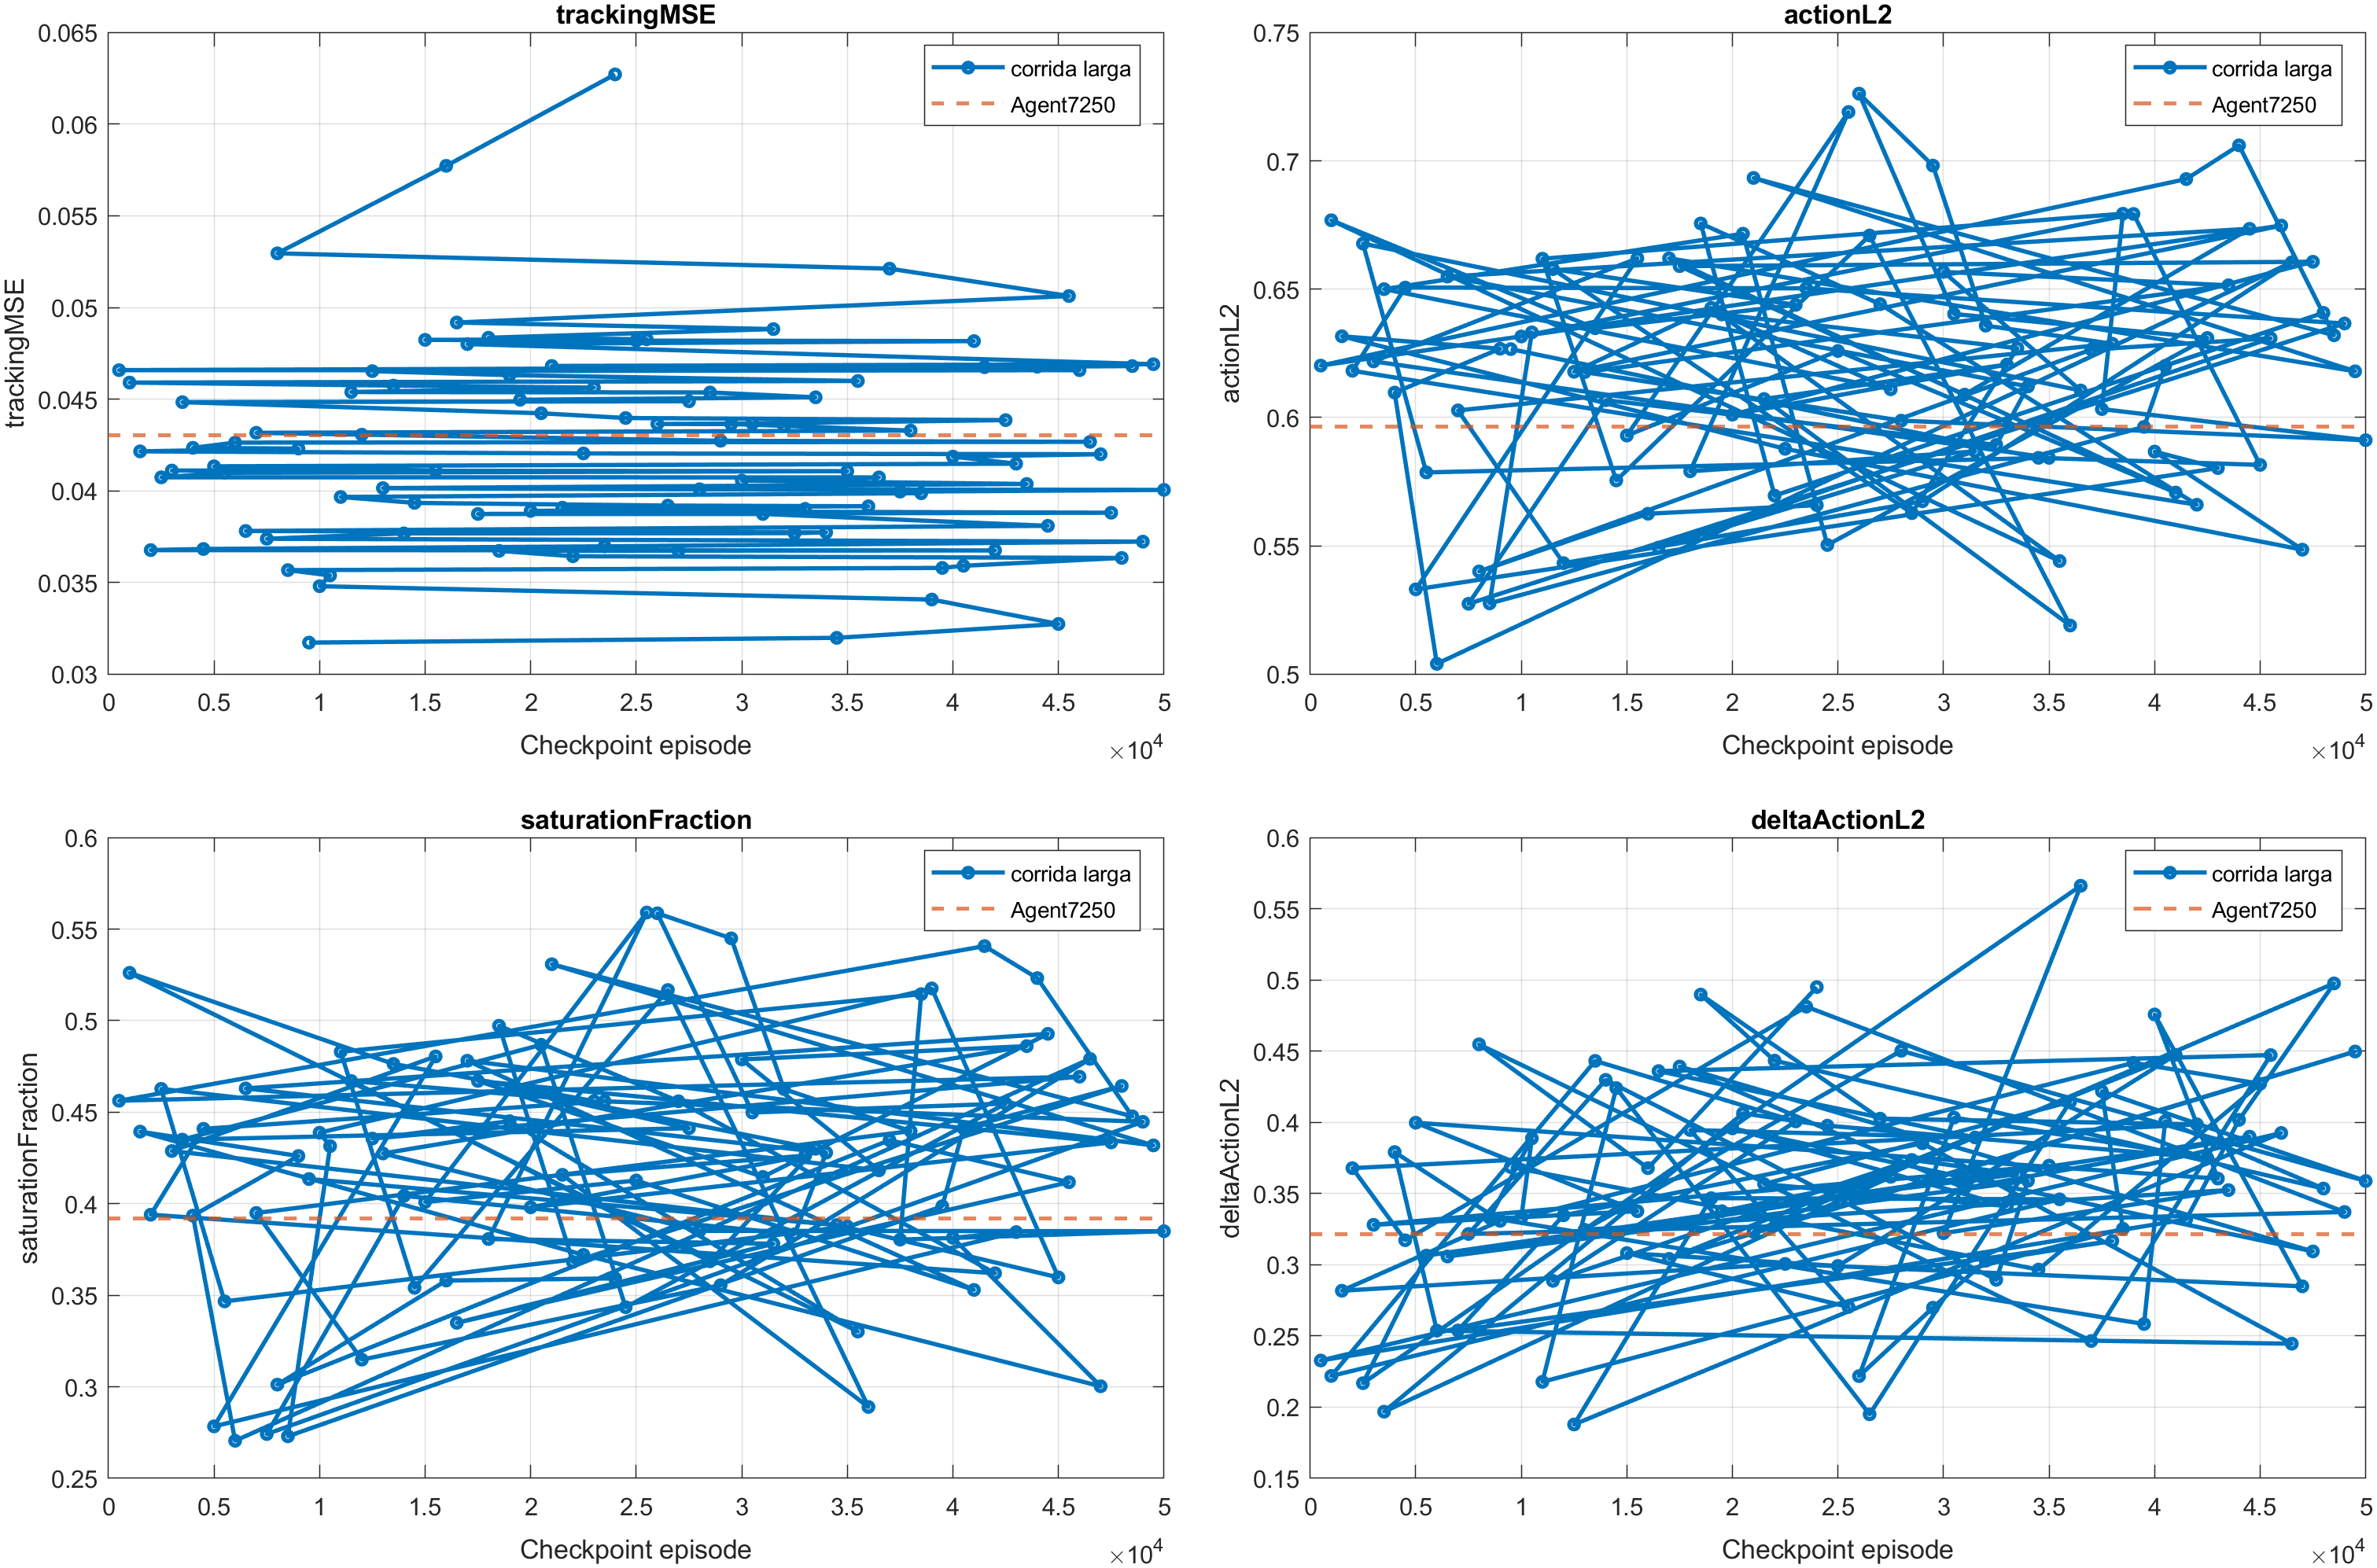
\includegraphics[width=\linewidth]{figures/longrun_residual_checkpoint_evolution_20260402.png}
\caption{Evoluci\'on de m\'etricas por checkpoint a lo largo de la corrida larga. La auditor\'ia completa sobre toda la trayectoria permite ver si entrenar m\'as ayud\'o, no cambi\'o o empeor\'o el compromiso final.}
\label{fig:audit}
\end{figure}

El mejor checkpoint seg\'un la auditor\'ia completa fue \texttt{Agent39000.mat}. Su resultado en la fase completa fue:
\begin{itemize}
    \item \texttt{trackingMSE = 0.041691}
    \item \texttt{actionL2 = 0.586194}
    \item \texttt{saturationFraction = 0.366878}
    \item \texttt{deltaActionL2 = 0.369051}
    \item estado: \texttt{ConditionA}
\end{itemize}

La Tabla~\ref{tab:phaseb} muestra los cinco mejores checkpoints de la fase completa.

\begin{table}[H]
\centering
\caption{Top 5 de la auditor\'ia completa (\texttt{phaseB})}
\label{tab:phaseb}
\begin{tabularx}{\linewidth}{l c c c c c}
\toprule
Checkpoint & Episodio & trackingMSE & actionL2 & saturation & Estado \\
\midrule
\texttt{Agent39000} & 39000 & 0.041691 & 0.586194 & 0.366878 & ConditionA \\
\texttt{Agent34500} & 34500 & 0.042154 & 0.588247 & 0.387136 & ConditionA \\
\texttt{Agent10000} & 10000 & 0.044034 & 0.601559 & 0.400134 & Rejected \\
\texttt{Agent9500} & 9500 & 0.044114 & 0.576220 & 0.355323 & Rejected \\
\texttt{Agent45000} & 45000 & 0.047300 & 0.584201 & 0.369649 & Rejected \\
\bottomrule
\end{tabularx}
\end{table}

Este punto es importante: la auditor\'ia s\'i encontr\'o checkpoints atractivos dentro de la corrida larga. El problema apareci\'o al hacer el retest independiente del mejor candidato.

\section*{Test final y comparaci\'on controlada}
El mejor checkpoint auditado, \texttt{Agent39000}, se volvi\'o a evaluar con 50 simulaciones y plots activados. Adem\'as, se ejecutaron tests comparativos equivalentes para:
\begin{itemize}
    \item \texttt{Agent7250} (benchmark oficial),
    \item \texttt{Agent1850} (mejor residual single-run hist\'orico),
    \item \texttt{seed 22} (mejor residual reproducible),
    \item \texttt{Agent39000} (mejor checkpoint de la corrida larga).
\end{itemize}

\begin{figure}[H]
\centering
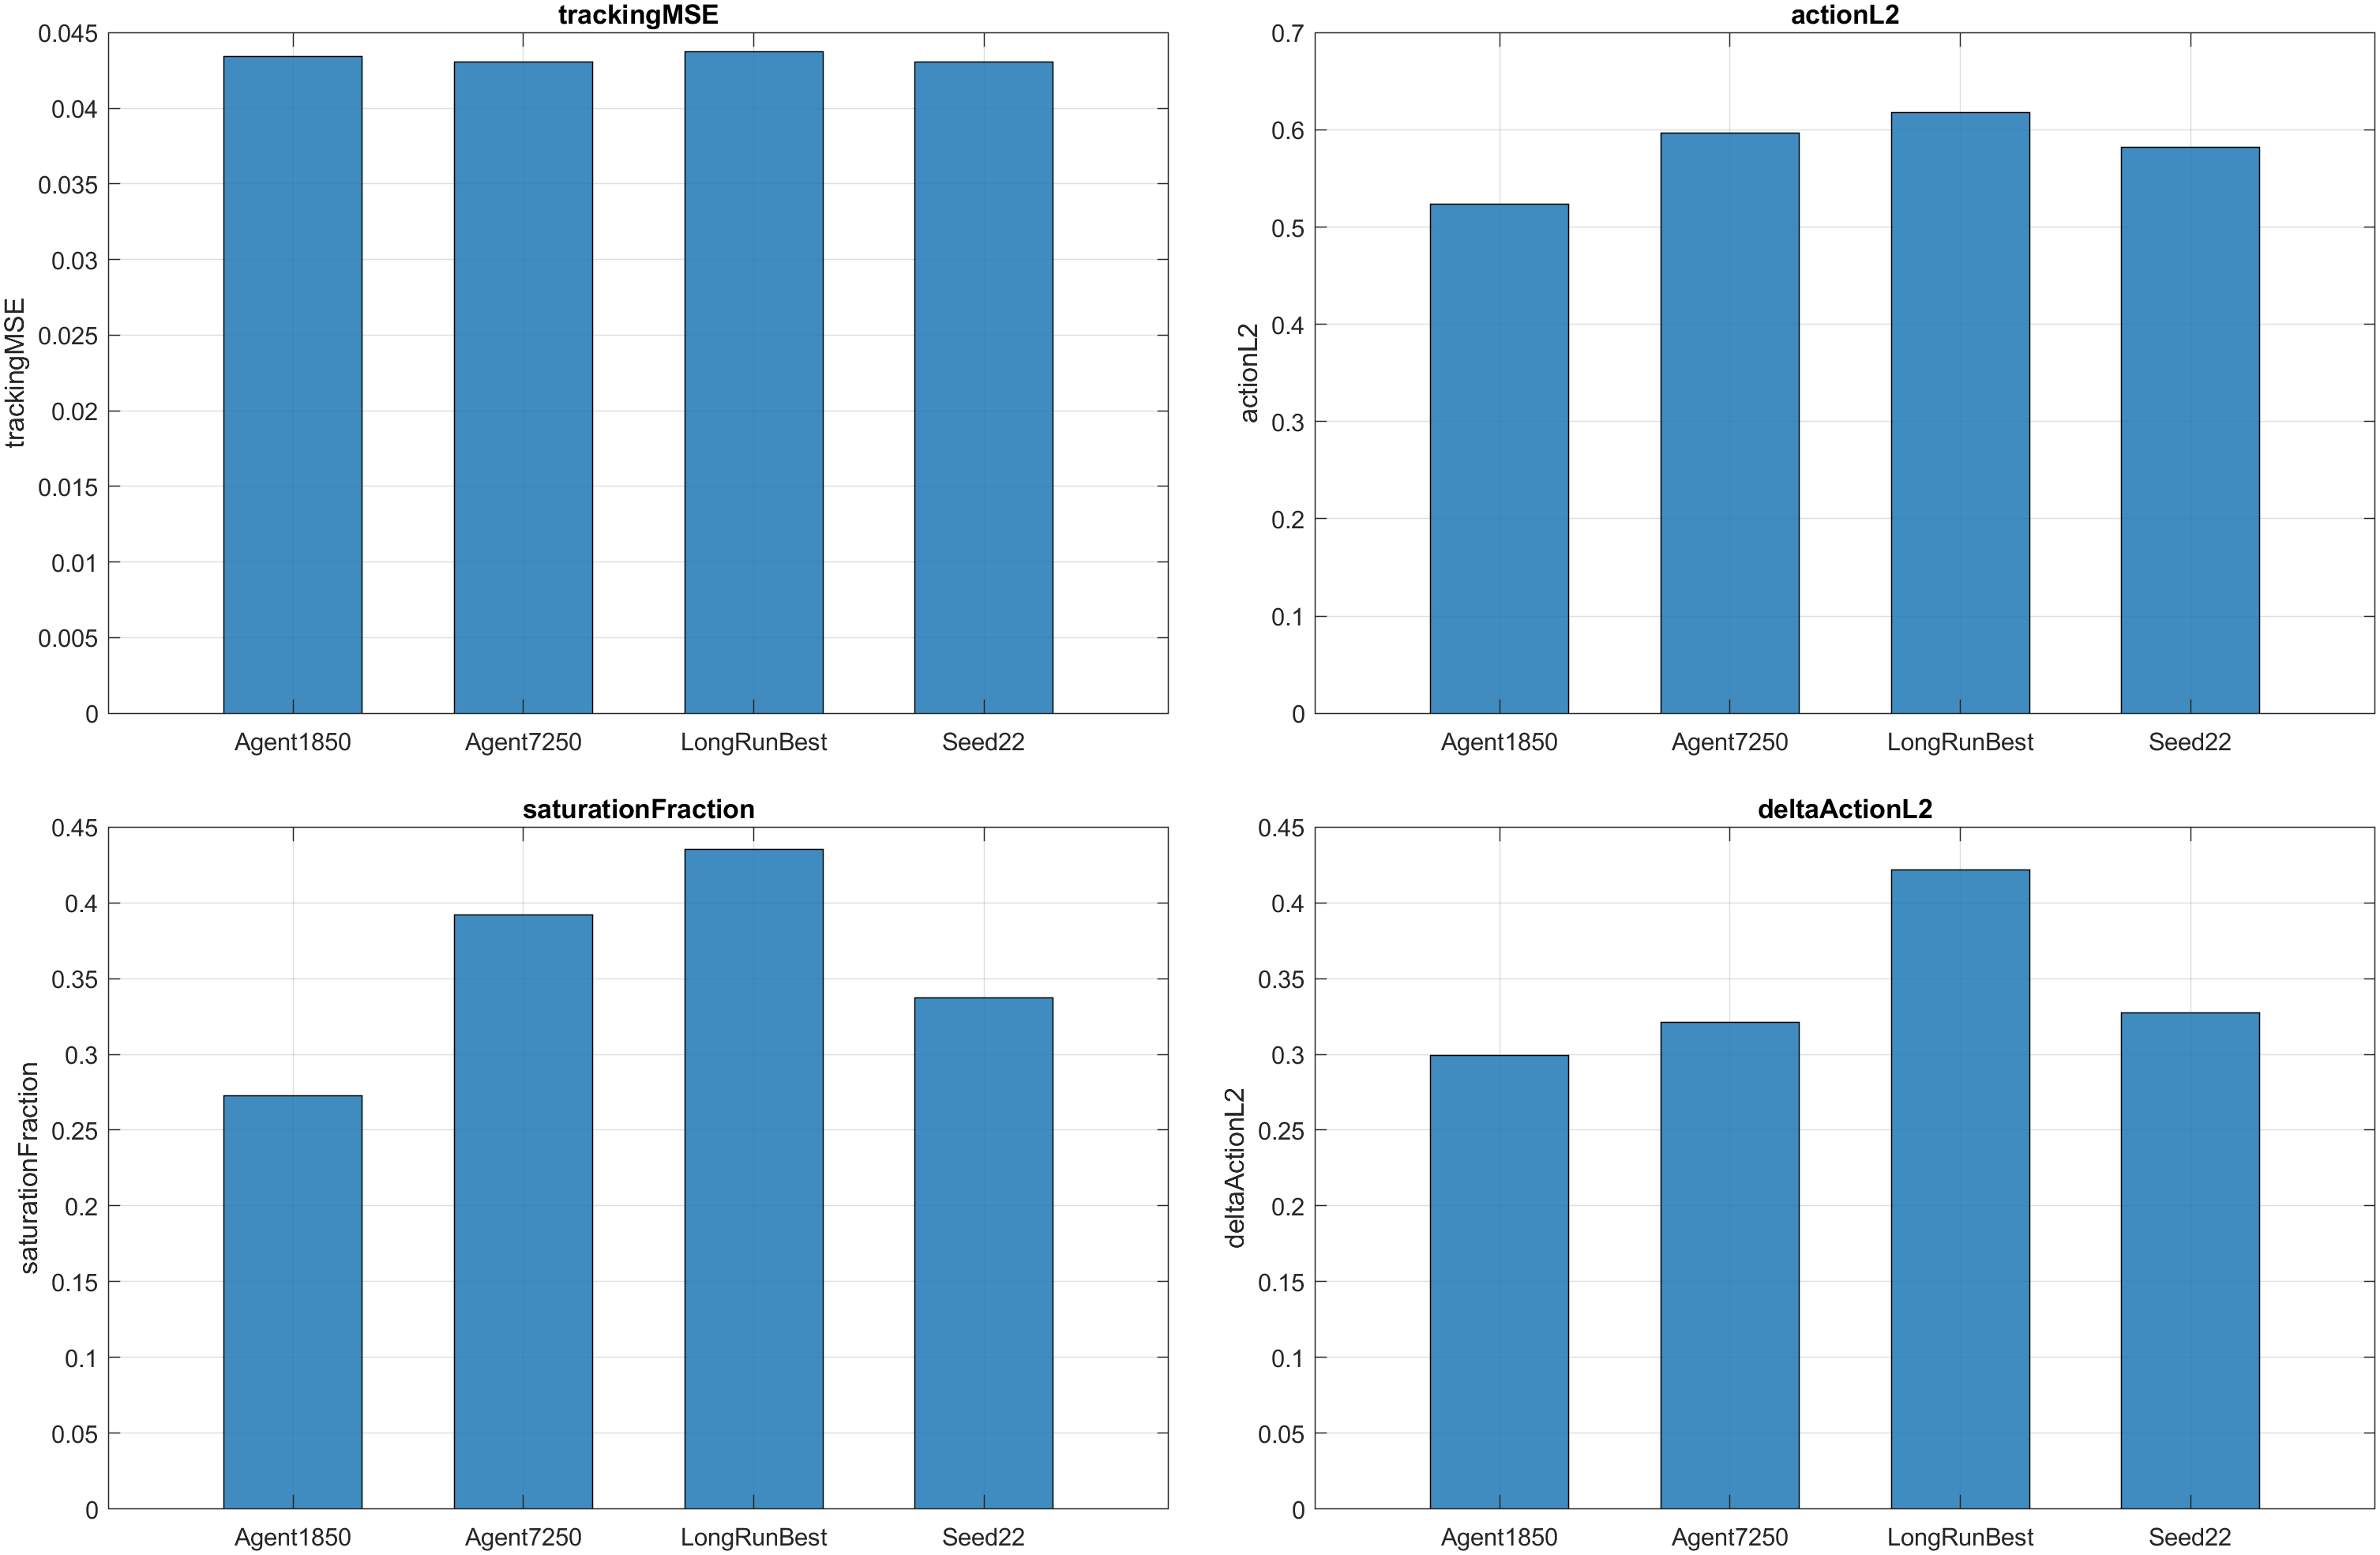
\includegraphics[width=\linewidth]{figures/longrun_residual_candidate_comparison_20260402.png}
\caption{Comparaci\'on final entre los cuatro candidatos relevantes del proyecto. La corrida larga se compara contra el benchmark oficial, el mejor residual single-run hist\'orico y la mejor seed reproducible.}
\label{fig:comparison}
\end{figure}

\begin{table}[H]
\centering
\caption{Comparaci\'on final entre benchmark, residuales previos y corrida larga}
\label{tab:final}
\small
\begin{tabularx}{\linewidth}{l c c c c c >{\raggedright\arraybackslash}p{2.25cm}}
\toprule
Candidato & trackingMSE & trackingMAE & actionL2 & saturation & deltaActionL2 & Estado frente al benchmark \\
\midrule
\texttt{Agent7250} & 0.043045 & 0.160336 & 0.596444 & 0.392086 & 0.321385 & Referencia \\
\texttt{Agent1850} & 0.043445 & 0.163542 & 0.523597 & 0.272637 & 0.299262 & ConditionB \\
\texttt{seed 22} & 0.043045 & 0.160786 & 0.582152 & 0.337475 & 0.327141 & ConditionA \\
\texttt{Agent39000} & 0.043727 & 0.161297 & 0.618205 & 0.435191 & 0.421769 & Rejected \\
\bottomrule
\end{tabularx}
\end{table}

La conclusi\'on del test final es m\'as dura que la de la auditor\'ia:
\begin{itemize}
    \item \texttt{Agent39000} empeor\'o el \texttt{trackingMSE} en aproximadamente \(+1.58\%\) frente a \texttt{Agent7250};
    \item tambi\'en empeor\'o \texttt{actionL2} en \(+3.65\%\);
    \item empeor\'o \texttt{saturationFraction} en \(+10.99\%\);
    \item y empeor\'o \texttt{deltaActionL2} en \(+31.23\%\).
\end{itemize}

Es decir, el mejor candidato encontrado dentro de la corrida larga \textbf{no sostuvo} su promesa cuando se lo reteste\'o con el mismo rigor final que se usa para tomar decisiones del proyecto.

\section*{Lectura visual del mejor checkpoint largo frente al benchmark}
La Fig.~\ref{fig:visuals} muestra un episodio representativo del mejor checkpoint largo y del benchmark can\'onico.

\begin{figure}[H]
\centering
\begin{minipage}[t]{0.49\linewidth}
\centering
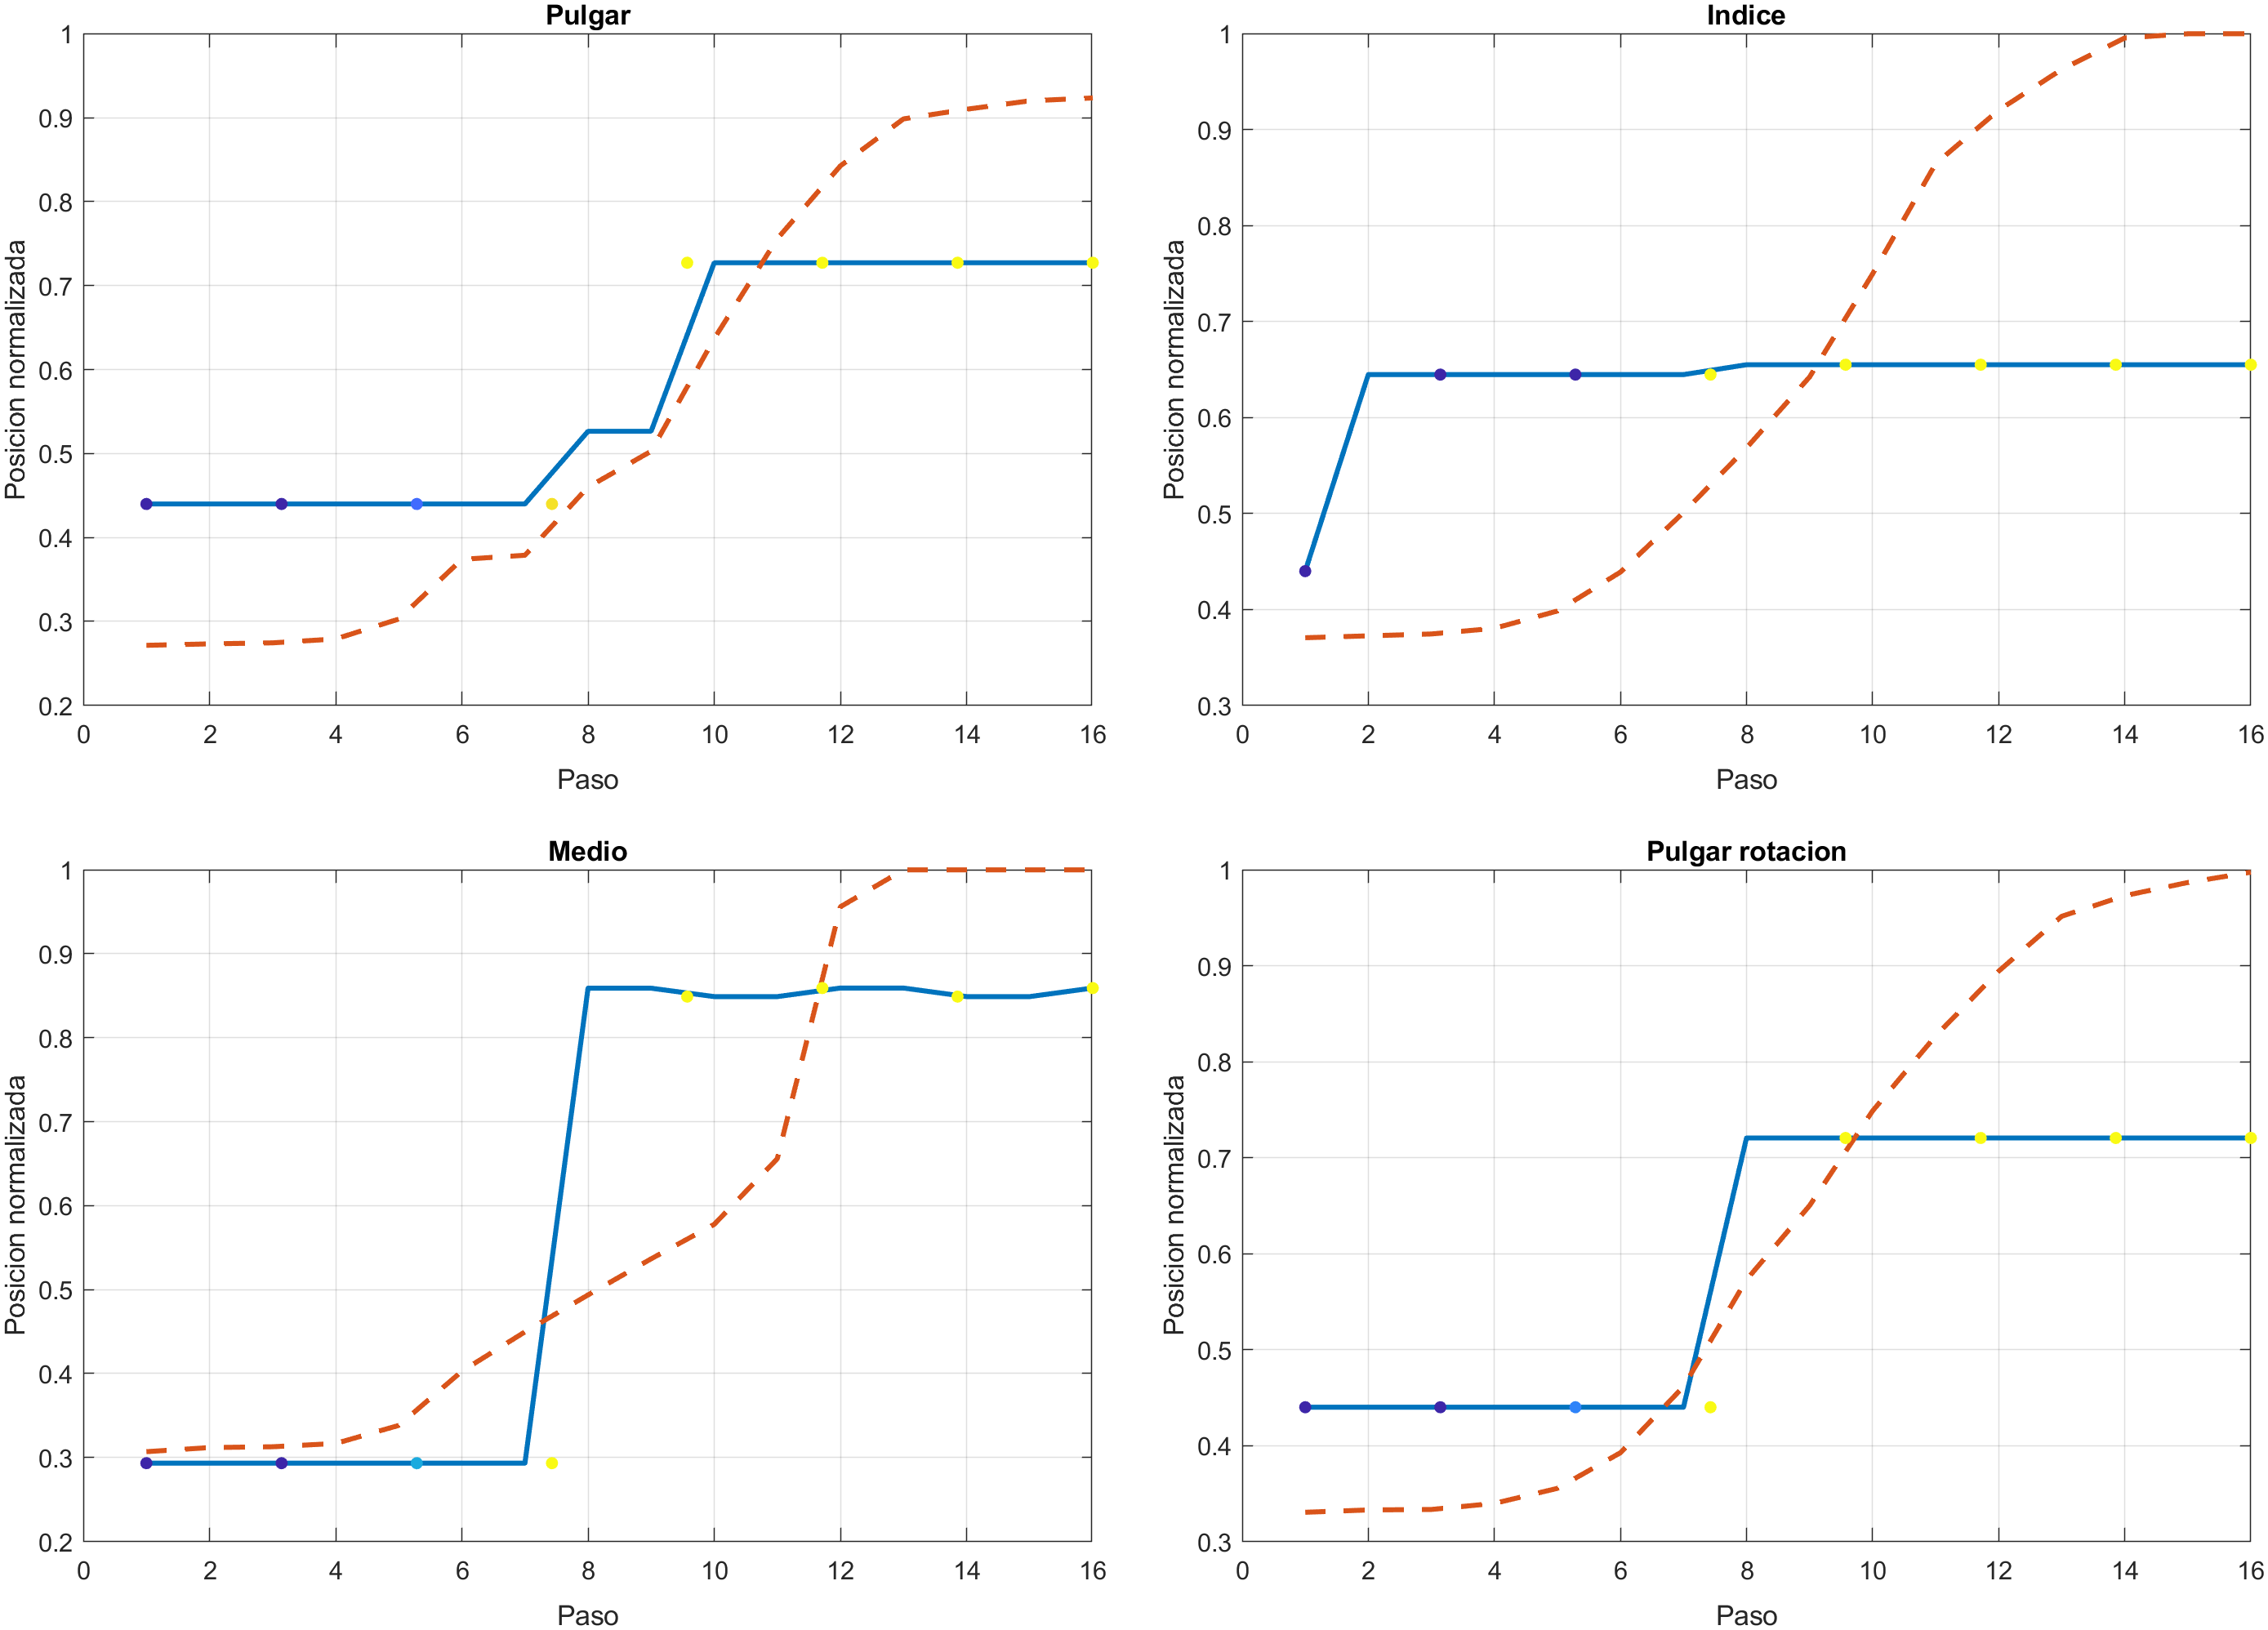
\includegraphics[width=\linewidth]{figures/longrun_residual_best_visual_20260402.png}
\caption*{(a) Mejor checkpoint largo: \texttt{Agent39000}}
\end{minipage}\hfill
\begin{minipage}[t]{0.49\linewidth}
\centering
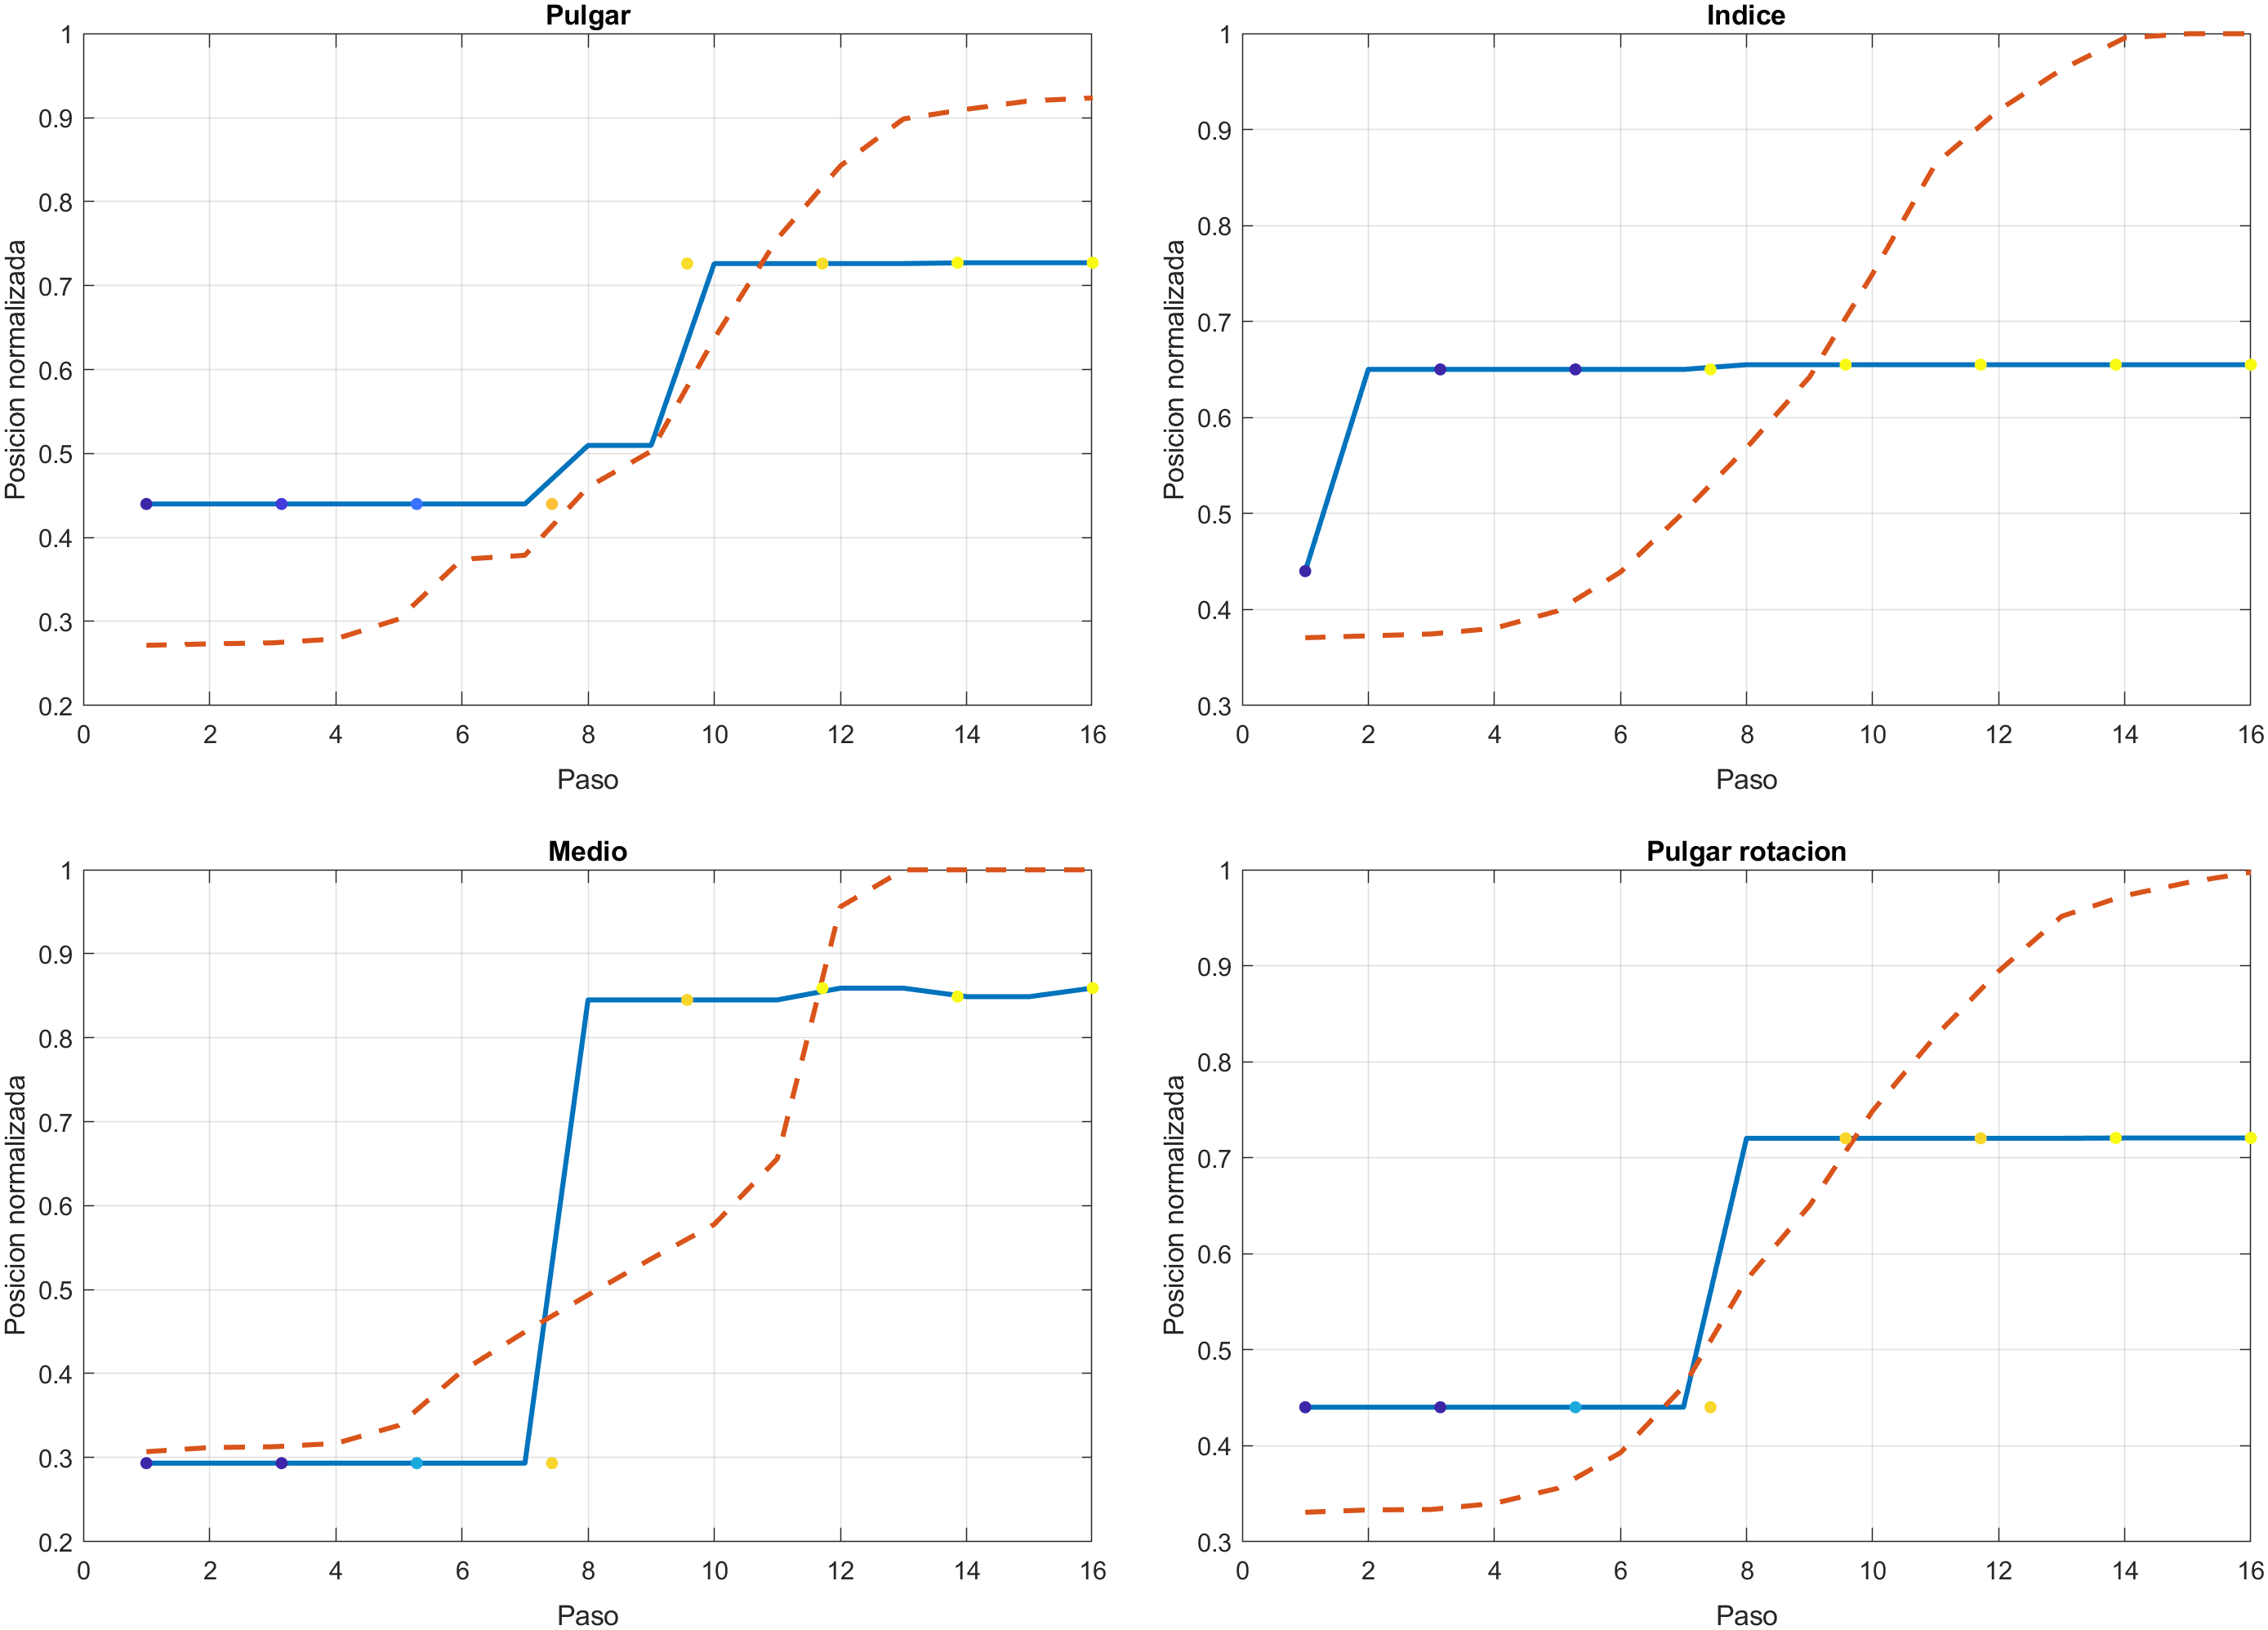
\includegraphics[width=\linewidth]{figures/longrun_residual_benchmark_visual_20260402.png}
\caption*{(b) Benchmark: \texttt{Agent7250}}
\end{minipage}
\caption{Comparaci\'on visual cualitativa entre el mejor checkpoint de la corrida larga y el benchmark oficial.}
\label{fig:visuals}
\end{figure}

A nivel de interpretaci\'on, estas figuras sirven como apoyo cualitativo, pero el veredicto se apoya principalmente en la tabla de m\'etricas y no en la inspecci\'on visual aislada.

\section*{Veredicto}
La corrida larga \textbf{no cambia el benchmark oficial del proyecto}. El resultado final de la auditor\'ia y el test comparativo obliga a mantener esta lectura:
\begin{itemize}
    \item \texttt{Agent7250} sigue siendo el \textbf{benchmark estable} del proyecto;
    \item la \texttt{seed 22} sigue siendo la \textbf{mejor referencia residual reproducible};
    \item \texttt{Agent1850} sigue siendo el \textbf{mejor residual single-run hist\'orico en compromiso esfuerzo/saturaci\'on};
    \item la corrida larga queda como \textbf{exploraci\'on temporal}, \'util para entender deriva y comportamiento futuro, pero sin promoci\'on a benchmark ni a nuevo l\'ider residual.
\end{itemize}

En otras palabras, entrenar mucho m\'as tiempo s\'i produjo checkpoints internamente prometedores, pero no produjo un candidato final mejor que los ya existentes cuando se aplic\'o el mismo protocolo de validaci\'on final.

\section*{En qu\'e punto estamos}
El estado actualizado del proyecto, despu\'es de esta auditor\'ia, es:
\begin{enumerate}
    \item el benchmark oficial sigue siendo \texttt{Agent7250};
    \item la l\'inea residual sigue siendo la intervenci\'on m\'as interesante, pero su evidencia fuerte est\'a en el mejor single-run y en una sola seed reproducible aceptada;
    \item la corrida larga no justific\'o reemplazar ese estado actual;
    \item el aprendizaje principal de esta extensi\'on es que \textbf{m\'as episodios no garantizan mejor pol\'itica final} y pueden inducir deriva tard\'ia.
\end{enumerate}

Por tanto, si se reabre esta l\'inea a futuro, la continuaci\'on m\'as sensata no es volver a empujar una sola corrida largu\'isima a ciegas, sino:
\begin{itemize}
    \item seleccionar mejor el punto de parada,
    \item usar auditor\'ias peri\'odicas m\'as frecuentes,
    \item o replantear la estabilidad del residual antes de volver a escalar episodios.
\end{itemize}

\section*{Conclusi\'on general}
La corrida larga cumpli\'o bien su funci\'on exploratoria: mostr\'o qu\'e ocurre cuando el residual se extiende hasta 50000 episodios y permiti\'o responder esa pregunta con datos reales, no con intuici\'on. El resultado principal es negativo en t\'erminos de promoci\'on de modelo, pero positivo como aprendizaje del proyecto: el residual no mejora simplemente por entrenarse durante mucho m\'as tiempo, y el mejor punto de compromiso puede aparecer bastante antes del final.

Esto deja una foto del proyecto m\'as clara y m\'as madura: \texttt{Agent7250} sigue como referencia estable, mientras que la corrida larga se documenta correctamente como experimento exploratorio de horizonte temporal extendido.

\end{document}
